\documentclass{standalone}
\usepackage{tikz}
\usetikzlibrary{patterns, positioning}
\usepackage[sfdefault]{ClearSans} %% option 'sfdefault' activates Clear Sans as the default text font
\usepackage[T1]{fontenc}

\begin{document}
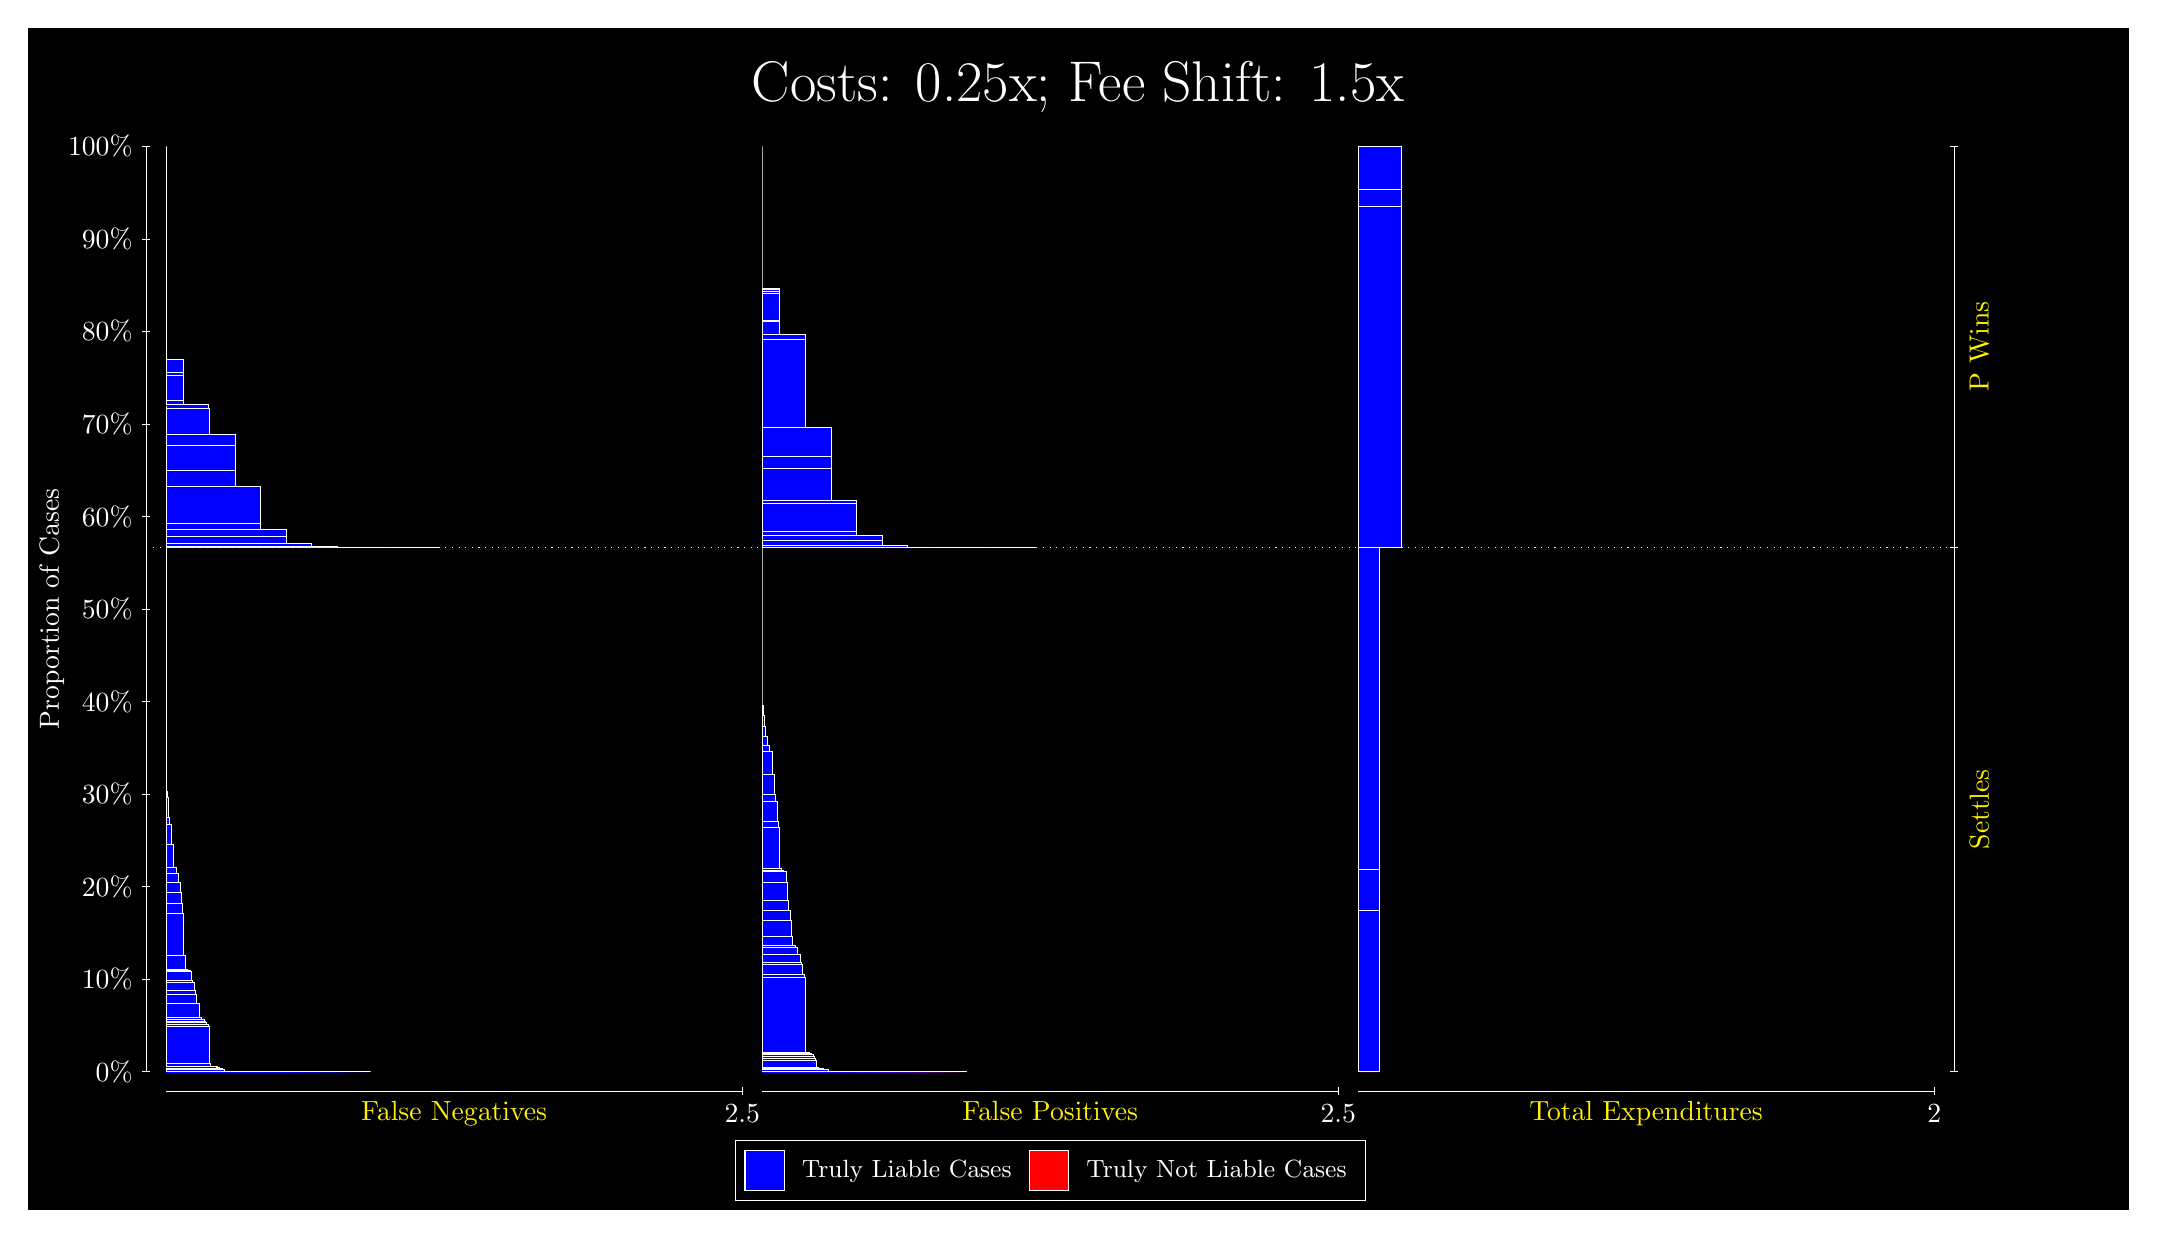
\begin{tikzpicture}
\draw[fill=black] (0,0) rectangle (26.667,15);
\draw[text=white] (0,13.5) rectangle (26.667,15) node[midway] {\huge Costs: 0.25x; Fee Shift: 1.5x};
\draw[white, very thin] (1.5,1.75) -- (1.5,13.5);
\node[rotate=90, text=white, anchor=center] at (0.3, 7.625) {Proportion of Cases};
\draw[white, very thin] (1.45,1.75) -- (1.55,1.75);
\node[text=white, anchor=east] at (1.45, 1.75) {0\%};
\draw[white, very thin] (1.45,2.925) -- (1.55,2.925);
\node[text=white, anchor=east] at (1.45, 2.925) {10\%};
\draw[white, very thin] (1.45,4.1) -- (1.55,4.1);
\node[text=white, anchor=east] at (1.45, 4.1) {20\%};
\draw[white, very thin] (1.45,5.275) -- (1.55,5.275);
\node[text=white, anchor=east] at (1.45, 5.275) {30\%};
\draw[white, very thin] (1.45,6.45) -- (1.55,6.45);
\node[text=white, anchor=east] at (1.45, 6.45) {40\%};
\draw[white, very thin] (1.45,7.625) -- (1.55,7.625);
\node[text=white, anchor=east] at (1.45, 7.625) {50\%};
\draw[white, very thin] (1.45,8.8) -- (1.55,8.8);
\node[text=white, anchor=east] at (1.45, 8.8) {60\%};
\draw[white, very thin] (1.45,9.975) -- (1.55,9.975);
\node[text=white, anchor=east] at (1.45, 9.975) {70\%};
\draw[white, very thin] (1.45,11.15) -- (1.55,11.15);
\node[text=white, anchor=east] at (1.45, 11.15) {80\%};
\draw[white, very thin] (1.45,12.325) -- (1.55,12.325);
\node[text=white, anchor=east] at (1.45, 12.325) {90\%};
\draw[white, very thin] (1.45,13.5) -- (1.55,13.5);
\node[text=white, anchor=east] at (1.45, 13.5) {100\%};

\draw[white, very thin] (24.457,1.75) -- (24.457,13.5);
\draw[white, very thin] (24.407,1.75) -- (24.507,1.75);
\node[anchor=west] at (24.407, 1.75) {};
\draw[white, very thin] (24.407,8.4106) -- (24.507,8.4106);
\node[anchor=west] at (24.407, 8.4106) {};
\draw[white, very thin] (24.407,13.5) -- (24.507,13.5);
\node[anchor=west] at (24.407, 13.5) {};

\draw[white, very thin, fill=blue] (1.75,1.75) rectangle (4.3482,1.75);
\draw[white, very thin, fill=blue] (1.75,1.75) rectangle (4.2018,1.75);
\draw[white, very thin, fill=blue] (1.75,1.75) rectangle (4.0554,1.75);
\draw[white, very thin, fill=blue] (1.75,1.75) rectangle (4.0229,1.75);
\draw[white, very thin, fill=blue] (1.75,1.75) rectangle (3.9091,1.75);
\draw[white, very thin, fill=blue] (1.75,1.75) rectangle (3.8765,1.75);
\draw[white, very thin, fill=blue] (1.75,1.75) rectangle (3.7627,1.75);
\draw[white, very thin, fill=blue] (1.75,1.75) rectangle (3.7302,1.75);
\draw[white, very thin, fill=blue] (1.75,1.75) rectangle (3.6976,1.75);
\draw[white, very thin, fill=blue] (1.75,1.75) rectangle (3.6163,1.75);
\draw[white, very thin, fill=blue] (1.75,1.75) rectangle (3.5838,1.75);
\draw[white, very thin, fill=blue] (1.75,1.75) rectangle (3.5513,1.75);
\draw[white, very thin, fill=blue] (1.75,1.75) rectangle (3.4699,1.75);
\draw[white, very thin, fill=blue] (1.75,1.75) rectangle (3.4374,1.75);
\draw[white, very thin, fill=blue] (1.75,1.75) rectangle (3.4049,1.75);
\draw[white, very thin, fill=blue] (1.75,1.75) rectangle (3.3723,1.75);
\draw[white, very thin, fill=blue] (1.75,1.75) rectangle (3.3236,1.75);
\draw[white, very thin, fill=blue] (1.75,1.75) rectangle (3.291,1.75);
\draw[white, very thin, fill=blue] (1.75,1.75) rectangle (3.2585,1.75);
\draw[white, very thin, fill=blue] (1.75,1.75) rectangle (3.226,1.75);
\draw[white, very thin, fill=blue] (1.75,1.75) rectangle (3.1772,1.75);
\draw[white, very thin, fill=blue] (1.75,1.75) rectangle (3.1447,1.75);
\draw[white, very thin, fill=blue] (1.75,1.75) rectangle (3.1121,1.75);
\draw[white, very thin, fill=blue] (1.75,1.75) rectangle (3.0796,1.75);
\draw[white, very thin, fill=blue] (1.75,1.75) rectangle (3.0471,1.75);
\draw[white, very thin, fill=blue] (1.75,1.75) rectangle (3.0308,1.75);
\draw[white, very thin, fill=blue] (1.75,1.75) rectangle (2.9983,1.75);
\draw[white, very thin, fill=blue] (1.75,1.75) rectangle (2.9657,1.75);
\draw[white, very thin, fill=blue] (1.75,1.75) rectangle (2.9332,1.75);
\draw[white, very thin, fill=blue] (1.75,1.75) rectangle (2.9007,1.75);
\draw[white, very thin, fill=blue] (1.75,1.75) rectangle (2.8844,1.75);
\draw[white, very thin, fill=blue] (1.75,1.75) rectangle (2.8519,1.7501);
\draw[white, very thin, fill=blue] (1.75,1.7501) rectangle (2.8194,1.7505);
\draw[white, very thin, fill=blue] (1.75,1.7505) rectangle (2.7868,1.7507);
\draw[white, very thin, fill=blue] (1.75,1.7507) rectangle (2.7543,1.7507);
\draw[white, very thin, fill=blue] (1.75,1.7507) rectangle (2.738,1.7507);
\draw[white, very thin, fill=blue] (1.75,1.7507) rectangle (2.7218,1.7508);
\draw[white, very thin, fill=blue] (1.75,1.7508) rectangle (2.7055,1.7509);
\draw[white, very thin, fill=blue] (1.75,1.7509) rectangle (2.673,1.7509);
\draw[white, very thin, fill=blue] (1.75,1.7509) rectangle (2.6405,1.7531);
\draw[white, very thin, fill=blue] (1.75,1.7531) rectangle (2.6079,1.7537);
\draw[white, very thin, fill=blue] (1.75,1.7537) rectangle (2.5917,1.7549);
\draw[white, very thin, fill=blue] (1.75,1.7549) rectangle (2.5754,1.7553);
\draw[white, very thin, fill=blue] (1.75,1.7553) rectangle (2.5591,1.756);
\draw[white, very thin, fill=blue] (1.75,1.756) rectangle (2.5266,1.7578);
\draw[white, very thin, fill=blue] (1.75,1.7578) rectangle (2.4941,1.7795);
\draw[white, very thin, fill=blue] (1.75,1.7795) rectangle (2.4616,1.7882);
\draw[white, very thin, fill=blue] (1.75,1.7882) rectangle (2.4453,1.7974);
\draw[white, very thin, fill=blue] (1.75,1.7974) rectangle (2.429,1.8034);
\draw[white, very thin, fill=blue] (1.75,1.8034) rectangle (2.4128,1.8054);
\draw[white, very thin, fill=blue] (1.75,1.8054) rectangle (2.3965,1.8106);
\draw[white, very thin, fill=blue] (1.75,1.8106) rectangle (2.3802,1.8134);
\draw[white, very thin, fill=blue] (1.75,1.8134) rectangle (2.3477,1.8162);
\draw[white, very thin, fill=blue] (1.75,1.8162) rectangle (2.3152,1.8607);
\draw[white, very thin, fill=blue] (1.75,1.8607) rectangle (2.2989,2.3248);
\draw[white, very thin, fill=blue] (1.75,2.3248) rectangle (2.2827,2.3466);
\draw[white, very thin, fill=blue] (1.75,2.3466) rectangle (2.2664,2.3714);
\draw[white, very thin, fill=blue] (1.75,2.3714) rectangle (2.2501,2.3903);
\draw[white, very thin, fill=blue] (1.75,2.3903) rectangle (2.2339,2.4099);
\draw[white, very thin, fill=blue] (1.75,2.4099) rectangle (2.2013,2.4389);
\draw[white, very thin, fill=blue] (1.75,2.4389) rectangle (2.1688,2.618);
\draw[white, very thin, fill=blue] (1.75,2.618) rectangle (2.1363,2.7312);
\draw[white, very thin, fill=blue] (1.75,2.7312) rectangle (2.12,2.7822);
\draw[white, very thin, fill=blue] (1.75,2.7822) rectangle (2.1037,2.8809);
\draw[white, very thin, fill=blue] (1.75,2.8809) rectangle (2.0875,2.9085);
\draw[white, very thin, fill=blue] (1.75,2.9085) rectangle (2.0712,3.0173);
\draw[white, very thin, fill=blue] (1.75,3.0173) rectangle (2.055,3.0349);
\draw[white, very thin, fill=blue] (1.75,3.0349) rectangle (2.0224,3.0526);
\draw[white, very thin, fill=blue] (1.75,3.0526) rectangle (1.9899,3.2305);
\draw[white, very thin, fill=blue] (1.75,3.2305) rectangle (1.9736,3.757);
\draw[white, very thin, fill=blue] (1.75,3.757) rectangle (1.9574,3.8894);
\draw[white, very thin, fill=blue] (1.75,3.8894) rectangle (1.9411,4.0213);
\draw[white, very thin, fill=blue] (1.75,4.0213) rectangle (1.9248,4.1591);
\draw[white, very thin, fill=blue] (1.75,4.1591) rectangle (1.9086,4.2726);
\draw[white, very thin, fill=blue] (1.75,4.2726) rectangle (1.876,4.3456);
\draw[white, very thin, fill=blue] (1.75,4.3456) rectangle (1.8435,4.6311);
\draw[white, very thin, fill=blue] (1.75,4.6311) rectangle (1.811,4.8893);
\draw[white, very thin, fill=blue] (1.75,4.8893) rectangle (1.7947,4.9763);
\draw[white, very thin, fill=blue] (1.75,4.9763) rectangle (1.7785,5.2377);
\draw[white, very thin, fill=blue] (1.75,5.2377) rectangle (1.7622,5.3064);
\draw[white, very thin, fill=red] (1.75,5.3064) rectangle (1.75,5.3064);
\draw[white, very thin, fill=blue] (1.75,5.3064) rectangle (1.75,8.4106);
\draw[white, very thin, fill=blue] (1.75,8.4106) rectangle (5.2265,8.4106);
\draw[white, very thin, fill=blue] (1.75,8.4106) rectangle (4.9012,8.4106);
\draw[white, very thin, fill=blue] (1.75,8.4106) rectangle (4.5759,8.4106);
\draw[white, very thin, fill=blue] (1.75,8.4106) rectangle (4.5759,8.4106);
\draw[white, very thin, fill=blue] (1.75,8.4106) rectangle (4.2506,8.4108);
\draw[white, very thin, fill=blue] (1.75,8.4108) rectangle (4.2506,8.411);
\draw[white, very thin, fill=blue] (1.75,8.411) rectangle (3.9253,8.4158);
\draw[white, very thin, fill=blue] (1.75,8.4158) rectangle (3.9172,8.4158);
\draw[white, very thin, fill=blue] (1.75,8.4158) rectangle (3.6,8.4532);
\draw[white, very thin, fill=blue] (1.75,8.4532) rectangle (3.5919,8.4532);
\draw[white, very thin, fill=blue] (1.75,8.4532) rectangle (3.2748,8.5475);
\draw[white, very thin, fill=blue] (1.75,8.5475) rectangle (3.2748,8.6368);
\draw[white, very thin, fill=blue] (1.75,8.6368) rectangle (3.2666,8.6368);
\draw[white, very thin, fill=blue] (1.75,8.6368) rectangle (3.2666,8.6368);
\draw[white, very thin, fill=blue] (1.75,8.6368) rectangle (2.9495,8.7108);
\draw[white, very thin, fill=blue] (1.75,8.7108) rectangle (2.9495,9.1808);
\draw[white, very thin, fill=blue] (1.75,9.1808) rectangle (2.9413,9.1808);
\draw[white, very thin, fill=blue] (1.75,9.1808) rectangle (2.9413,9.1808);
\draw[white, very thin, fill=blue] (1.75,9.1808) rectangle (2.6242,9.3814);
\draw[white, very thin, fill=blue] (1.75,9.3814) rectangle (2.6242,9.7094);
\draw[white, very thin, fill=blue] (1.75,9.7094) rectangle (2.6242,9.8454);
\draw[white, very thin, fill=blue] (1.75,9.8454) rectangle (2.6161,9.8461);
\draw[white, very thin, fill=blue] (1.75,9.8461) rectangle (2.6161,9.8461);
\draw[white, very thin, fill=blue] (1.75,9.8461) rectangle (2.6161,9.8464);
\draw[white, very thin, fill=blue] (1.75,9.8464) rectangle (2.2989,10.178);
\draw[white, very thin, fill=blue] (1.75,10.178) rectangle (2.2908,10.178);
\draw[white, very thin, fill=blue] (1.75,10.178) rectangle (2.2908,10.22);
\draw[white, very thin, fill=blue] (1.75,10.22) rectangle (1.9736,10.221);
\draw[white, very thin, fill=blue] (1.75,10.221) rectangle (1.9736,10.271);
\draw[white, very thin, fill=blue] (1.75,10.271) rectangle (1.9736,10.272);
\draw[white, very thin, fill=blue] (1.75,10.272) rectangle (1.9655,10.598);
\draw[white, very thin, fill=blue] (1.75,10.598) rectangle (1.9655,10.629);
\draw[white, very thin, fill=blue] (1.75,10.629) rectangle (1.9655,10.793);
\draw[white, very thin, fill=red] (1.75,10.793) rectangle (1.75,10.793);
\draw[white, very thin, fill=blue] (1.75,10.793) rectangle (1.75,13.5);
\draw[white, very thin, fill=red] (9.3189,1.75) rectangle (11.917,1.75);
\draw[white, very thin, fill=blue] (9.3189,1.75) rectangle (11.917,1.75);
\draw[white, very thin, fill=red] (9.3189,1.75) rectangle (11.771,1.75);
\draw[white, very thin, fill=blue] (9.3189,1.75) rectangle (11.771,1.75);
\draw[white, very thin, fill=red] (9.3189,1.75) rectangle (11.624,1.75);
\draw[white, very thin, fill=blue] (9.3189,1.75) rectangle (11.624,1.75);
\draw[white, very thin, fill=blue] (9.3189,1.75) rectangle (11.592,1.75);
\draw[white, very thin, fill=red] (9.3189,1.75) rectangle (11.478,1.75);
\draw[white, very thin, fill=blue] (9.3189,1.75) rectangle (11.478,1.75);
\draw[white, very thin, fill=blue] (9.3189,1.75) rectangle (11.445,1.75);
\draw[white, very thin, fill=red] (9.3189,1.75) rectangle (11.332,1.75);
\draw[white, very thin, fill=blue] (9.3189,1.75) rectangle (11.332,1.75);
\draw[white, very thin, fill=blue] (9.3189,1.75) rectangle (11.299,1.75);
\draw[white, very thin, fill=blue] (9.3189,1.75) rectangle (11.266,1.75);
\draw[white, very thin, fill=red] (9.3189,1.75) rectangle (11.185,1.75);
\draw[white, very thin, fill=blue] (9.3189,1.75) rectangle (11.185,1.75);
\draw[white, very thin, fill=blue] (9.3189,1.75) rectangle (11.153,1.75);
\draw[white, very thin, fill=blue] (9.3189,1.75) rectangle (11.12,1.75);
\draw[white, very thin, fill=red] (9.3189,1.75) rectangle (11.039,1.75);
\draw[white, very thin, fill=blue] (9.3189,1.75) rectangle (11.039,1.75);
\draw[white, very thin, fill=blue] (9.3189,1.75) rectangle (11.006,1.75);
\draw[white, very thin, fill=blue] (9.3189,1.75) rectangle (10.974,1.75);
\draw[white, very thin, fill=blue] (9.3189,1.75) rectangle (10.941,1.75);
\draw[white, very thin, fill=red] (9.3189,1.75) rectangle (10.892,1.75);
\draw[white, very thin, fill=blue] (9.3189,1.75) rectangle (10.892,1.75);
\draw[white, very thin, fill=blue] (9.3189,1.75) rectangle (10.86,1.75);
\draw[white, very thin, fill=blue] (9.3189,1.75) rectangle (10.827,1.75);
\draw[white, very thin, fill=blue] (9.3189,1.75) rectangle (10.795,1.75);
\draw[white, very thin, fill=red] (9.3189,1.75) rectangle (10.746,1.75);
\draw[white, very thin, fill=blue] (9.3189,1.75) rectangle (10.746,1.75);
\draw[white, very thin, fill=blue] (9.3189,1.75) rectangle (10.714,1.75);
\draw[white, very thin, fill=blue] (9.3189,1.75) rectangle (10.681,1.75);
\draw[white, very thin, fill=blue] (9.3189,1.75) rectangle (10.648,1.75);
\draw[white, very thin, fill=blue] (9.3189,1.75) rectangle (10.616,1.75);
\draw[white, very thin, fill=red] (9.3189,1.75) rectangle (10.6,1.75);
\draw[white, very thin, fill=blue] (9.3189,1.75) rectangle (10.6,1.75);
\draw[white, very thin, fill=blue] (9.3189,1.75) rectangle (10.567,1.75);
\draw[white, very thin, fill=blue] (9.3189,1.75) rectangle (10.535,1.75);
\draw[white, very thin, fill=blue] (9.3189,1.75) rectangle (10.502,1.75);
\draw[white, very thin, fill=blue] (9.3189,1.75) rectangle (10.47,1.75);
\draw[white, very thin, fill=red] (9.3189,1.75) rectangle (10.453,1.75);
\draw[white, very thin, fill=blue] (9.3189,1.75) rectangle (10.453,1.7502);
\draw[white, very thin, fill=blue] (9.3189,1.7502) rectangle (10.421,1.7502);
\draw[white, very thin, fill=blue] (9.3189,1.7502) rectangle (10.388,1.7502);
\draw[white, very thin, fill=blue] (9.3189,1.7502) rectangle (10.356,1.7507);
\draw[white, very thin, fill=blue] (9.3189,1.7507) rectangle (10.323,1.7512);
\draw[white, very thin, fill=red] (9.3189,1.7512) rectangle (10.307,1.7512);
\draw[white, very thin, fill=blue] (9.3189,1.7512) rectangle (10.307,1.7524);
\draw[white, very thin, fill=blue] (9.3189,1.7524) rectangle (10.291,1.7529);
\draw[white, very thin, fill=blue] (9.3189,1.7529) rectangle (10.274,1.7534);
\draw[white, very thin, fill=blue] (9.3189,1.7534) rectangle (10.242,1.7535);
\draw[white, very thin, fill=blue] (9.3189,1.7535) rectangle (10.209,1.7535);
\draw[white, very thin, fill=blue] (9.3189,1.7535) rectangle (10.177,1.7552);
\draw[white, very thin, fill=red] (9.3189,1.7552) rectangle (10.161,1.7552);
\draw[white, very thin, fill=blue] (9.3189,1.7552) rectangle (10.161,1.7734);
\draw[white, very thin, fill=blue] (9.3189,1.7734) rectangle (10.144,1.7752);
\draw[white, very thin, fill=blue] (9.3189,1.7752) rectangle (10.128,1.7822);
\draw[white, very thin, fill=blue] (9.3189,1.7822) rectangle (10.095,1.7871);
\draw[white, very thin, fill=blue] (9.3189,1.7871) rectangle (10.063,1.7889);
\draw[white, very thin, fill=blue] (9.3189,1.7889) rectangle (10.03,1.8062);
\draw[white, very thin, fill=red] (9.3189,1.8062) rectangle (10.014,1.8062);
\draw[white, very thin, fill=blue] (9.3189,1.8062) rectangle (10.014,1.8992);
\draw[white, very thin, fill=blue] (9.3189,1.8992) rectangle (9.9979,1.9192);
\draw[white, very thin, fill=blue] (9.3189,1.9192) rectangle (9.9816,1.9442);
\draw[white, very thin, fill=blue] (9.3189,1.9442) rectangle (9.9654,1.9679);
\draw[white, very thin, fill=blue] (9.3189,1.9679) rectangle (9.9491,1.9871);
\draw[white, very thin, fill=blue] (9.3189,1.9871) rectangle (9.9166,1.9899);
\draw[white, very thin, fill=blue] (9.3189,1.9899) rectangle (9.884,1.9926);
\draw[white, very thin, fill=red] (9.3189,1.9926) rectangle (9.8678,1.9926);
\draw[white, very thin, fill=blue] (9.3189,1.9926) rectangle (9.8678,2.9515);
\draw[white, very thin, fill=blue] (9.3189,2.9515) rectangle (9.8515,2.9788);
\draw[white, very thin, fill=blue] (9.3189,2.9788) rectangle (9.8353,3.1087);
\draw[white, very thin, fill=blue] (9.3189,3.1087) rectangle (9.819,3.1387);
\draw[white, very thin, fill=blue] (9.3189,3.1387) rectangle (9.8027,3.2385);
\draw[white, very thin, fill=blue] (9.3189,3.2385) rectangle (9.7702,3.3262);
\draw[white, very thin, fill=blue] (9.3189,3.3262) rectangle (9.7377,3.3551);
\draw[white, very thin, fill=blue] (9.3189,3.3551) rectangle (9.7051,3.4657);
\draw[white, very thin, fill=blue] (9.3189,3.4657) rectangle (9.6889,3.6694);
\draw[white, very thin, fill=blue] (9.3189,3.6694) rectangle (9.6726,3.7971);
\draw[white, very thin, fill=blue] (9.3189,3.7971) rectangle (9.6563,3.9312);
\draw[white, very thin, fill=blue] (9.3189,3.9312) rectangle (9.6401,4.1559);
\draw[white, very thin, fill=blue] (9.3189,4.1559) rectangle (9.6238,4.2924);
\draw[white, very thin, fill=blue] (9.3189,4.2924) rectangle (9.5913,4.3101);
\draw[white, very thin, fill=blue] (9.3189,4.3101) rectangle (9.5588,4.3277);
\draw[white, very thin, fill=blue] (9.3189,4.3277) rectangle (9.5425,4.8542);
\draw[white, very thin, fill=blue] (9.3189,4.8542) rectangle (9.5262,4.9229);
\draw[white, very thin, fill=blue] (9.3189,4.9229) rectangle (9.51,5.1843);
\draw[white, very thin, fill=blue] (9.3189,5.1843) rectangle (9.4937,5.2713);
\draw[white, very thin, fill=blue] (9.3189,5.2713) rectangle (9.4774,5.5295);
\draw[white, very thin, fill=blue] (9.3189,5.5295) rectangle (9.4449,5.815);
\draw[white, very thin, fill=blue] (9.3189,5.815) rectangle (9.4124,5.888);
\draw[white, very thin, fill=blue] (9.3189,5.888) rectangle (9.3799,6.0015);
\draw[white, very thin, fill=blue] (9.3189,6.0015) rectangle (9.3636,6.1392);
\draw[white, very thin, fill=blue] (9.3189,6.1392) rectangle (9.3473,6.2712);
\draw[white, very thin, fill=blue] (9.3189,6.2712) rectangle (9.3311,6.4036);
\draw[white, very thin, fill=blue] (9.3189,6.4036) rectangle (9.3189,8.4106);
\draw[white, very thin, fill=red] (9.3189,8.4106) rectangle (12.795,8.4106);
\draw[white, very thin, fill=blue] (9.3189,8.4106) rectangle (12.795,8.4106);
\draw[white, very thin, fill=red] (9.3189,8.4106) rectangle (12.47,8.4106);
\draw[white, very thin, fill=blue] (9.3189,8.4106) rectangle (12.47,8.4106);
\draw[white, very thin, fill=red] (9.3189,8.4106) rectangle (12.145,8.4106);
\draw[white, very thin, fill=blue] (9.3189,8.4106) rectangle (12.145,8.4106);
\draw[white, very thin, fill=blue] (9.3189,8.4106) rectangle (12.145,8.4106);
\draw[white, very thin, fill=blue] (9.3189,8.4106) rectangle (11.819,8.4107);
\draw[white, very thin, fill=red] (9.3189,8.4107) rectangle (11.819,8.4107);
\draw[white, very thin, fill=blue] (9.3189,8.4107) rectangle (11.819,8.4108);
\draw[white, very thin, fill=red] (9.3189,8.4108) rectangle (11.494,8.4108);
\draw[white, very thin, fill=blue] (9.3189,8.4108) rectangle (11.494,8.413);
\draw[white, very thin, fill=red] (9.3189,8.413) rectangle (11.486,8.413);
\draw[white, very thin, fill=blue] (9.3189,8.413) rectangle (11.486,8.413);
\draw[white, very thin, fill=red] (9.3189,8.413) rectangle (11.169,8.413);
\draw[white, very thin, fill=blue] (9.3189,8.413) rectangle (11.169,8.4346);
\draw[white, very thin, fill=red] (9.3189,8.4346) rectangle (11.161,8.4346);
\draw[white, very thin, fill=blue] (9.3189,8.4346) rectangle (11.161,8.4346);
\draw[white, very thin, fill=blue] (9.3189,8.4346) rectangle (10.844,8.4983);
\draw[white, very thin, fill=red] (9.3189,8.4983) rectangle (10.844,8.4983);
\draw[white, very thin, fill=blue] (9.3189,8.4983) rectangle (10.844,8.5594);
\draw[white, very thin, fill=red] (9.3189,8.5594) rectangle (10.835,8.5594);
\draw[white, very thin, fill=blue] (9.3189,8.5594) rectangle (10.835,8.5594);
\draw[white, very thin, fill=blue] (9.3189,8.5594) rectangle (10.835,8.5594);
\draw[white, very thin, fill=blue] (9.3189,8.5594) rectangle (10.518,8.6078);
\draw[white, very thin, fill=red] (9.3189,8.6078) rectangle (10.518,8.6078);
\draw[white, very thin, fill=blue] (9.3189,8.6078) rectangle (10.518,8.9655);
\draw[white, very thin, fill=blue] (9.3189,8.9655) rectangle (10.518,9.0027);
\draw[white, very thin, fill=blue] (9.3189,9.0027) rectangle (10.51,9.0027);
\draw[white, very thin, fill=red] (9.3189,9.0027) rectangle (10.51,9.0027);
\draw[white, very thin, fill=blue] (9.3189,9.0027) rectangle (10.51,9.0027);
\draw[white, very thin, fill=blue] (9.3189,9.0027) rectangle (10.193,9.4073);
\draw[white, very thin, fill=blue] (9.3189,9.4073) rectangle (10.193,9.5594);
\draw[white, very thin, fill=blue] (9.3189,9.5594) rectangle (10.193,9.9371);
\draw[white, very thin, fill=blue] (9.3189,9.9371) rectangle (10.185,9.9371);
\draw[white, very thin, fill=red] (9.3189,9.9371) rectangle (10.185,9.9371);
\draw[white, very thin, fill=blue] (9.3189,9.9371) rectangle (10.185,9.9371);
\draw[white, very thin, fill=blue] (9.3189,9.9371) rectangle (9.8678,11.046);
\draw[white, very thin, fill=blue] (9.3189,11.046) rectangle (9.8678,11.118);
\draw[white, very thin, fill=blue] (9.3189,11.118) rectangle (9.8597,11.118);
\draw[white, very thin, fill=red] (9.3189,11.118) rectangle (9.8597,11.118);
\draw[white, very thin, fill=blue] (9.3189,11.118) rectangle (9.8597,11.118);
\draw[white, very thin, fill=blue] (9.3189,11.118) rectangle (9.5425,11.282);
\draw[white, very thin, fill=blue] (9.3189,11.282) rectangle (9.5425,11.297);
\draw[white, very thin, fill=blue] (9.3189,11.297) rectangle (9.5425,11.639);
\draw[white, very thin, fill=blue] (9.3189,11.639) rectangle (9.5344,11.64);
\draw[white, very thin, fill=blue] (9.3189,11.64) rectangle (9.5344,11.655);
\draw[white, very thin, fill=red] (9.3189,11.655) rectangle (9.5344,11.655);
\draw[white, very thin, fill=blue] (9.3189,11.655) rectangle (9.5344,11.69);
\draw[white, very thin, fill=blue] (9.3189,11.69) rectangle (9.5344,11.691);
\draw[white, very thin, fill=red] (9.3189,11.691) rectangle (9.3189,11.691);
\draw[white, very thin, fill=blue] (9.3189,11.691) rectangle (9.3189,13.5);
\draw[white, very thin, fill=red] (16.888,1.75) rectangle (17.162,1.75);
\draw[white, very thin, fill=blue] (16.888,1.75) rectangle (17.162,3.8032);
\draw[white, very thin, fill=red] (16.888,3.8032) rectangle (17.162,3.8032);
\draw[white, very thin, fill=blue] (16.888,3.8032) rectangle (17.162,4.3176);
\draw[white, very thin, fill=red] (16.888,4.3176) rectangle (17.162,4.3176);
\draw[white, very thin, fill=blue] (16.888,4.3176) rectangle (17.162,8.4106);
\draw[white, very thin, fill=red] (16.888,8.4106) rectangle (17.437,8.4106);
\draw[white, very thin, fill=blue] (16.888,8.4106) rectangle (17.437,12.736);
\draw[white, very thin, fill=red] (16.888,12.736) rectangle (17.437,12.736);
\draw[white, very thin, fill=blue] (16.888,12.736) rectangle (17.437,12.953);
\draw[white, very thin, fill=red] (16.888,12.953) rectangle (17.437,12.953);
\draw[white, very thin, fill=blue] (16.888,12.953) rectangle (17.437,13.5);
\draw[white, dotted] (1.5,8.4106) -- (24.457,8.4106);
\draw[white, very thin] (1.75,1.5) -- (9.0689,1.5);
\node[text=yellow, anchor=north] at (5.4094, 1.5) {False Negatives};
\draw[white, very thin] (9.0689,1.45) -- (9.0689,1.55);
\node[text=white, anchor=north] at (9.0689, 1.45) {2.5};

\draw[white, very thin] (9.3189,1.5) -- (16.638,1.5);
\node[text=yellow, anchor=north] at (12.978, 1.5) {False Positives};
\draw[white, very thin] (16.638,1.45) -- (16.638,1.55);
\node[text=white, anchor=north] at (16.638, 1.45) {2.5};

\draw[white, very thin] (16.888,1.5) -- (24.207,1.5);
\node[text=yellow, anchor=north] at (20.547, 1.5) {Total Expenditures};
\draw[white, very thin] (24.207,1.45) -- (24.207,1.55);
\node[text=white, anchor=north] at (24.207, 1.45) {2};

\node[text=yellow, centered, rotate=90] at (24.777, 5.0803) {Settles};
\node[text=yellow, centered, rotate=90] at (24.777, 10.955) {P Wins};

\draw (12.978300999999998,1.5) node[draw=none] (baseCoordinate) {};
\begin{scope}[align=center]
        \matrix[scale=0.5, draw=white, below=0.5cm of baseCoordinate, nodes={draw}, column sep=0.1cm]{
            \node[rectangle, draw, minimum width=0.5cm, minimum height=0.5cm, fill=blue] {}; &
            \node[draw=none, font=\small, text=white] (B) {Truly Liable Cases}; &
            \node[rectangle, draw, minimum width=0.5cm, minimum height=0.5cm, fill=red] {}; &
            \node[draw=none, font=\small, text=white] (B) {Truly Not Liable Cases}; \\
            };
\end{scope}

\end{tikzpicture}
\end{document}